%Porting Viterbi Powerpoint template to beamer template
%author: sraok
%email: kuppanna@usc.edu
%Preamble
\documentclass{beamer}

\usepackage{default}
\usetheme{default}
\usecolortheme{dove}

%Defining viterbi template colors
\definecolor{viterbiyellow}{HTML}{E9A000}
\definecolor{viterbired}{HTML}{990000}

%Redefine more fields as required
\newcommand{\viterbititle}[1]{\title{\textcolor{viterbiyellow}{#1}}}
\newcommand{\viterbiauthor}[1]{\author{\textcolor{viterbiyellow}{#1}}}
\newcommand{\viterbidate}[1]{\date{\textcolor{viterbiyellow}{#1}}}

%Change this environment to include any additional formatting required
\newenvironment{viterbiframe}[1]{
\begin{frame}{\textcolor{viterbired}{#1}}
}
{\end{frame}}

%To show the outline slide before each section
\AtBeginSection[]
{
  \begin{viterbiframe}{Outline}
    \tableofcontents[currentsection,currentsubsection]
  \end{viterbiframe}
}






% %end preamble
%Document Begins here
\begin{document}




%Title slide

\viterbititle{Porting Viterbi Powerpoint template to latex/beamer}

\viterbiauthor{Sanmukh Rao Kuppannagari}
\viterbidate{March 6, 2015}

\setbeamertemplate{background}{
\includegraphics[height=\paperheight]{title}}


\begin{frame}
\titlepage
\end{frame}

\setbeamertemplate{background}{
\includegraphics[height=\paperheight]{template}}
%Table of contents
%Each \section or \subsection command in the document generates a TOC entry
\begin{viterbiframe}{Outline}
\tableofcontents
\end{viterbiframe}

%the document can be split in terms of sections or slides. I would prefer section level as a good tradeoff between number of tex files and complexity of each slide.
\section{This is First Section}


\begin{viterbiframe}{{Frame Title}}
\begin{itemize}
\item This is the text actually being shown
\item This is the way to create bullets
\item A lot of text is commented
\end{itemize}
\end{viterbiframe}

\begin{viterbiframe}{Another frame title}

\begin{columns}
\begin{column}{0.7\textwidth}
\begin{enumerate}
\item This is a way to create columns
\item Also to create numbered items
\end{enumerate}
\end{column}
\begin{column}{0.3\textwidth}
\begin{figure}
\centering
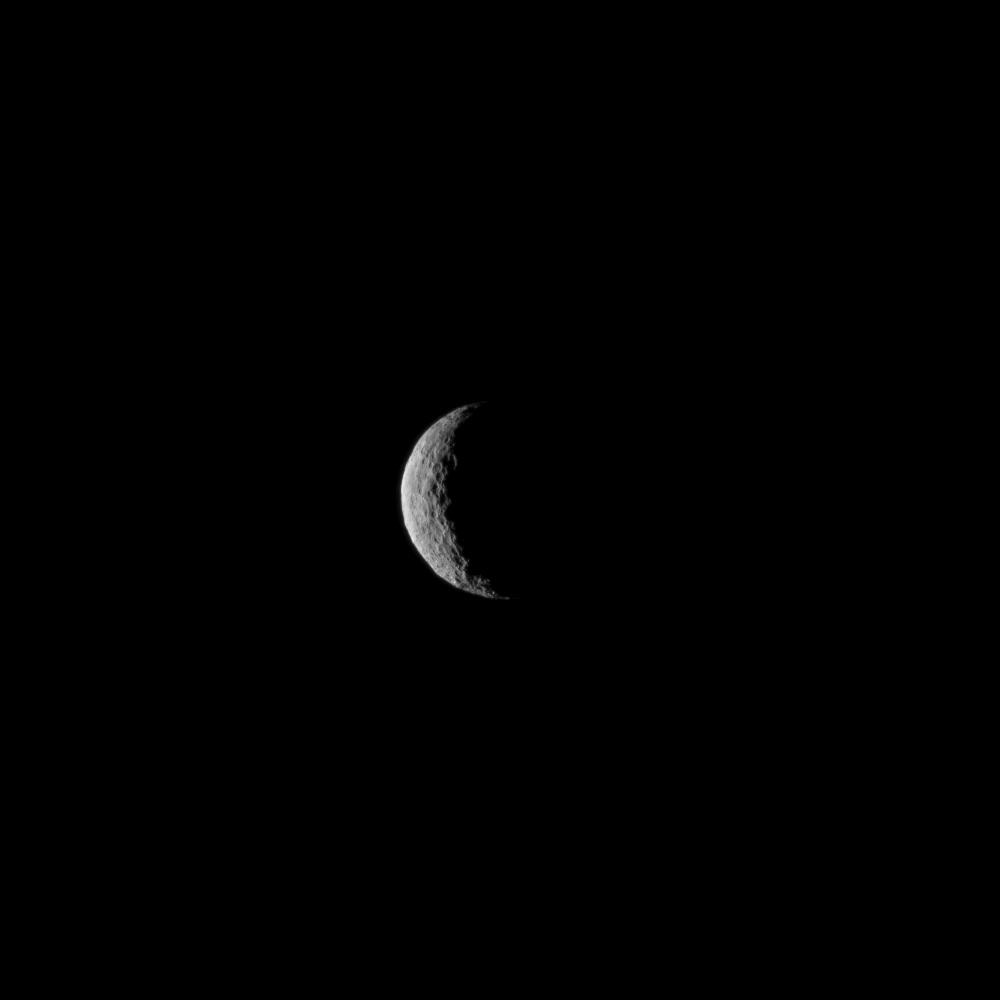
\includegraphics[width=0.9\linewidth]{./Ceres_Seen_From_NASA_s_Dawn_Spacecraft.jpg}
\caption{}
\label{fig:overiew_cnn}
\end{figure}
\end{column}
\end{columns}


\end{viterbiframe}
%\begin{frame}{Overview}
%
%\begin{columns}
%\begin{column}{0.7\textwidth}
%\begin{itemize}
%\item Computation Layer performs the convolution operation corresponding to a single layer 
%\item Time Multiplexed to implement various layers
%\item Input feature map read from DRAM
%\item Output feature map written to DRAM
%\item On-chip buffers for caching
%\item Interconnections from buffers to computation layers 
%\end{itemize}
%\end{column}
%
%\begin{column}{0.3\textwidth}
%\begin{figure}
%\centering
%\includegraphics[width=0.9\linewidth]{./overview_cnn}
%\caption{}
%\label{fig:overiew_cnn}
%\end{figure}
%\end{column}
%
%\end{columns}
%\end{frame} %end Overview
%
%\begin{frame}{Approach}
%\begin{itemize}
%\item Define computation stage optimizations and identify parameters
%\item Define communication reduction optimizations and identify parameters
%\item Generate performance model for Computation to communication ratio using the above parameters
%\item Performance design space exploration and generate optimized design defined by the values of the parameters
%\end{itemize}
%\end{frame}
%
%
%\begin{frame}[fragile]{Unoptimized Code}
%
%\begin{columns}
%\begin{column}{0.5\textwidth}
%\tiny
%\begin{verbatim}
%
%for(row=0; row < R; row++) {
%  for(col=0; col < C; col++) {
%    for(to=0; to < M; to++) {
%      for(ti=0; ti < N; ti++) {
%      //load output feature maps
%      //load weights
%      //load input feature maps
%        for(i=0; i < K; i++) {
%          for(j=0; j < K; j++) {
%            output_fm[to][row][column] +=
%               weights[to][ti]][i][j]*
%               input_fm[ti][S*row+i][S*col+j]; 
%        } }
%      //store output feature maps 
%
%} } } } 
%
%\end{verbatim}
%\end{column}
%\begin{column}{0.5\textwidth}
%\begin{itemize}
%\item Constants:
%\begin{itemize}
%\item Number of input feature maps $N$
%\item Number of output feature maps $M$
%\item Number of row in feature map in pixels $R$
%\item Number of columns in feature map in pixels $C$
%\item Kernel Size $K$
%\item Stride $S$
%\end{itemize}
%\end{itemize}
%
%\end{column}
%
%\end{columns}
%
%\end{frame}
%
%
%
%\begin{frame}{Computation Layer Optimizations}
%\begin{itemize}
%\item Loop Tiling: Partition loops into small chunks for data reuse 
%\item Loop Unrolling: Increase throughput at the cost of increased resources utilization
%\item Loop Pipelining: Overlap execution of operations from different loop iterations
%\end{itemize}
%\end{frame}
%
%\begin{frame}[fragile]{Loop Tiled Code}
%\vskip-1cm
%\tiny
%\begin{verbatim}
%for(row=0; row < R; row++) {
%  for(col=0; col < C; col++) {
%    for(to=0; to < M; to++) {
%      for(ti=0; ti < N; ti++) {
%      //load output feature maps
%      //load weights
%      //load input feature maps
%      
%      // on−chip data computation
%      for(trr=row;trr<min(row+Tr,R);trr++){
%        for(tcc=col;tcc<min(col+Tc,C);tcc++){
%          for(too=to;too<min(to+Tm,M);too++){
%            for(tii=ti;tii<min(ti+Tn,N);tii++){
%              for(i=0;i<K;i++){
%                for(j=0;j<K;j++){ 
%                  L:outputfm[too][trr][tcc]+=
%                      weights[too][tii][i][j]*
%                      inputfm[tii][S*trr+i][S*tcc+j];
%          
%       } } } } } }
%      //store output feature maps 
%
%} } } } 
%
%\end{verbatim}
%\vspace{-0.4in}
%\small
%\begin{itemize}
%\item Parameters $T_r, T_c, T_m, T_n$
%\end{itemize}
%
%\end{frame}
%
%\begin{frame}{Loop Unrolling}
%\vskip-0.5cm
%\begin{itemize}
%\item Loops across various dimensions can be unrolled to various degree
%\item Unrolling loops in different dimensions determine buffer to computation stage interconnect complexity
%\item Data sharing relations between different loop iterations of a loop dimension on a given Array $A$ can be: Irrelevant, Independent and Dependent
%\end{itemize}
%\vskip-0.5cm
%\begin{columns}
%\begin{column}{0.3\textwidth}
%\begin{figure}
%\centering
%\includegraphics[width=0.7\linewidth]{./loop_unrolling_irrelevant}
%\caption{Irrelevant}
%\label{fig:loop_unrolling_irrelevant}
%\end{figure}
%
%\end{column}
%
%\begin{column}{0.3\textwidth}
%\begin{figure}
%\centering
%\includegraphics[width=0.7\linewidth]{./loop_unrolling_independent}
%\caption{Independent}
%\label{fig:loop_unrolling_independent}
%\end{figure}\end{column}
%
%\begin{column}{0.3\textwidth}
%\begin{figure}
%\centering
%\includegraphics[width=0.7\linewidth]{./loop_unrolling_dependent}
%\caption{Dependent}
%\label{fig:loop_unrolling_dependent}
%\end{figure}
%\end{column}
%\end{columns}
%
%
%\end{frame}
%
%\begin{frame}[fragile]{Loop Unrolled and Pipelined Code}
%\vskip-0.5cm
%\begin{columns}
%\begin{column}{0.4\textwidth}
%\begin{itemize}
%\item Loops fully pipelined
%\item Loop dimensions $T_m$ and $T_n$ are fully unrolled
%\end{itemize}
%\end{column}
%
%\begin{column}{0.6\textwidth}
%\tiny
%\begin{verbatim}
%
%for(row=0; row < R; row++) {
%  for(col=0; col < C; col++) {
%    for(to=0; to < M; to++) {
%      for(ti=0; ti < N; ti++) {
%      //load output feature maps
%      //load weights
%      //load input feature maps
%      
%      // on−chip data computation
%      for(trr=row;trr<min(row+Tr,R);trr++){
%        for(tcc=col;tcc<min(col+Tc,C);tcc++){
%          for(too=to;too<min(to+Tm,M);too++){
%#pragma HLS UNROLL
%            for(tii=ti;tii<min(ti+Tn,N);tii++){
%#pragma HLS UNROLL
%              for(i=0;i<K;i++){
%                for(j=0;j<K;j++){ 
%                  L:outputfm[too][trr][tcc]+=
%                      weights[too][tii][i][j]*
%                      inputfm[tii][S*trr+i][S*tcc+j];
%          
%       } } } } } }
%      //store output feature maps 
%
%} } } } 
%
%\end{verbatim}
%\end{column}
%\end{columns}
%\end{frame}
%
%\begin{frame}[fragile]{Communication Optimizationed Code}
%\vskip-0.7cm
%\begin{columns}
%\begin{column}{0.4\textwidth}
%\begin{itemize}
%\item Move "Store output feature maps" outside the for loop corresponding to dimension: $tii$
%\end{itemize}
%\end{column}
%\begin{column}{0.6\textwidth}
%\tiny
%\begin{verbatim}
%
%for(row=0; row < R; row++) {
%  for(col=0; col < C; col++) {
%    for(to=0; to < M; to++) {
%      for(ti=0; ti < N; ti++) {
%      //load weights
%      //load input feature maps
%      
%      // on−chip data computation
%      for(trr=row;trr<min(row+Tr,R);trr++){
%        for(tcc=col;tcc<min(col+Tc,C);tcc++){
%          for(too=to;too<min(to+Tm,M);too++){
%#pragma HLS UNROLL
%            for(tii=ti;tii<min(ti+Tn,N);tii++){
%#pragma HLS UNROLL
%              for(i=0;i<K;i++){
%                for(j=0;j<K;j++){ 
%                  L:outputfm[too][trr][tcc]+=
%                      weights[too][tii][i][j]*
%                      inputfm[tii][S*trr+i][S*tcc+j];
%          
%       } } } } } }
%       
%
%      }
%      //store output feature maps 
%
%} } } 
%
%\end{verbatim}
%
%\end{column}
%\end{columns}
%
%\end{frame}
%
%\begin{frame}{Optimized Architecture}
%\begin{figure}
%\centering
%\includegraphics[width=0.7\linewidth]{./final}
%\caption{Optimized Architecture}
%\label{fig:final}
%\end{figure}
%
%\end{frame}
%
%
%\begin{frame}{Performance Model}
%\begin{itemize}
%\item Computation Roof
%\begin{math}
%~ \frac{2\times M \times N}{\lceil \frac{M}{T_m} \rceil + \lceil \frac{N}{T_n} \rceil}  
%\end{math}
%\item CTC Ratio
%\begin{math}
%\frac{2 \times R \times C \times M \times N \times K \times K}{\alpha_{in} \times \beta_{in} + \alpha_{wt} \times \beta_{wt} + \alpha_{out} \times \beta_{out}}
%\end{math}
%\item Where:
%\begin{itemize}
%\item $\alpha$ is trip counts
%\begin{math}
%\alpha_{in} = \alpha_{wt} = \frac{M}{T_m} \times \frac{N}{T_n} \times \frac{R}{T_r} \times \frac{C}{T_c}
%\alpha_{out}  = \frac{M}{T_m} \times  \frac{R}{T_r} \times \frac{C}{T_c}
%\end{math}
%\item $\beta$ is buffer size
%\end{itemize}
%
%\end{itemize}
%\end{frame}
%
%\begin{frame}{Experimental Results}
%\begin{itemize}
%\item Target Platform: Virtex 7
%\item Computation Roof: $T_m \times T_n =$ 100 GFLOPS 
%\item Optimal Design: $T_m = 64, T_n = 7, T_r = ?, T_c = ?$
%\item Bandwidth requirement: 2.2 GB/s
%\item Performance: 61.62 GFLOPS
%\item No DRAM configuration specified
%\end{itemize}
%\end{frame}

\section{This is Second section}

\begin{viterbiframe}{Frame 1}
\vskip5cm
\begin{itemize}
\item This slide shows how to add vertical space
\end{itemize}
\end{viterbiframe}



%\input{slide3.tex}

\end{document}
